\documentclass{classes/sice-si}


% \title{
% 	カーリングスキップロボットに関する研究 ~第一報:LRFとカメラを用いたストーン検出とシステムのROS化~
% }

% \author{
% 	〇熊本涼介,Trinh Quang Phi,曽根忠瑛,河村隆
% }

% タイトルと著者名
\title{カーリングストーンデリバリロボットにおける回転付加機構に関する検討と実装} % 和文タイトル
\name{○伊與田一,曽根忠瑛,河村隆(信州大学)} % 著者名
\etitle{Study and Implementation of Rotational Addition Mechanism in Curling Stone Delivery Robot} % 英文タイトル
\ename{○Hajime IYODA,Tadaaki SONE and Takashi KAWAMURA \\Shinshu University}	%著者名(英)


\setlength\textfloatsep{0pt} % 図と本文の間のスペース
\setlength\floatsep{0pt} % 図同士の間のスペース
\setlength\intextsep{0pt} % 図と本文の間のスペース(本文中の図の場合)

\begin{document}

% アブストラクト
\abst{We are developing a curling stone delivery robot that can make pitches that can be played against humans.
To enable reliable rotation, we are designing a mechanism to rotate the stone using the handle of the curling stone.
}
    % 人間と対戦可能な投球を行うカーリングストーンデリバリロボットの開発を行っている.
% 確実な回転を可能にするために,カーリングストーンのハンドルを使い,ストーンを回転させる機構を設計を行う.


\maketitle

\section{緒言}
本研究は,カーリング競技を対象とする.
% カーリング競技は,1998 年の長野大会からオリ
% ンピックの正式競技に採用され,2022 年の北京オリンピックにて,日本史上初となる銀メダ
% ルを獲得し ,日本国内でも広く認知される有名競技となった.
% しかし,
% カーリング競技は,ウィンタースポーツ全体で見ると,日本における競技人口は2020 年の調査では,
% 登録競技者が全体で2306 人と少なく\cite{key},また施設の普及の点においても他の競技には及ば
% ない,その理由として競技の理解が進んでいないことが原因の一つとして挙げられる.
カーリングは「氷上のチェス」と呼ばれ,細かい戦略,高度な技術を要するスポーツである.
氷の状態を読みストーンの投球を行うことは人の経験や感覚に頼る
ことが多く,戦略も大まかな定石しか存在しない.
% また,カーリングが行える環境が少ないことも普及の妨げになっていると考える.
% % 日本カーリング協会によると,カーリング専用施
% % 設は2024 年現在で日本に13 箇所しかなく,通年で使用可能な施設は8 箇所に限られる.
% 試合が行われるフィールド(カーリングシート)にも,製作や整備(アイスメイク)にも専
% 門的な技術を要する
本研究の目的は,人間と対戦可能なカーリングロボットシステムを開発することで,新たな戦略や未だに解明されていないストーンの挙動に関する物理現象を解明し,カーリング競技の普及・発展に寄与することである.

\section{デリバリロボット}
デリバリロボットは2つの主要な機構で構成されている.
1つ目は、カーリングストーンを目標速度で投球を行う押出機構である。
2つ目は、投球されるストーンに指定された回転を付与する回転付加機構である。
本報では,デリバリロボットにおける回転付加機構に関する検討と実装について述べる.
\section{回転付加機構について}
回転付加機構は,ストーンに角速度を与える機構であり,目標角速度は約12 rpmである.
% ストーンに回転を与えることにより,ストーンはカール(曲がる)する.


\subsection{先行研究について}
これまでに開発された回転付加機構について述べる.
今までのデリバリロボット試作機では,打ち出し時にストーンの外周円筒に対して押し付け、平ベルトで回転力を与える平ベルト式\cite{ref:sankou}と,ウレタンローラをストーンに押し付けて回転を付与するウレタンローラ式、平ベルト式を改良したタイミングベルト式が試作された.
% 開発された回転付加機構のCAD図を図\ref{fig:one} ~ 図\ref{fig:three}に示す.
% \begin{itemize}
%     \item 平ベルト方式  \cite{ref:sankou}
%     % モータに取り付けられたプーリで平ベルトを駆動させ,ストーンを押し出した際にベルトとストーンが接触し,摩擦によってストーンを回転させる
%     \item ウレタンローラ方式 
%     % モータに取り付けられたウレタンローラでストーンを回転させ,ストーンを回転させる.
%     \item タイミングベルト方式 
%     % 平ベルト式を参考にし開発され,問題を解決するために開発された.
%     % モータに取り付けられたプーリでタイミングベルトを駆動させ,ストーンを押し出した際にベルトとストーンが接触し,摩擦によってストーンを回転させる
% \end{itemize}
しかし,先行研究の回転付加機構には問題がある。
ベルト式ではベルトの摩擦により回転を与えるが、ベルトが滑ってしまい確実な回転ができていない問題やウレタンローラ式では回転付加機構の
強度不足という問題がある.
この問題解決のため,ストーンへの確実な回転を与え、強度が十分である新たな回転付加機構の開発が必要である.
% \begin{figure}[h]
%     \centering
%     \vspace{4pt} % 上部の余白を0に設定
%     \begin{minipage}{0.4\linewidth}
%         \centering
%         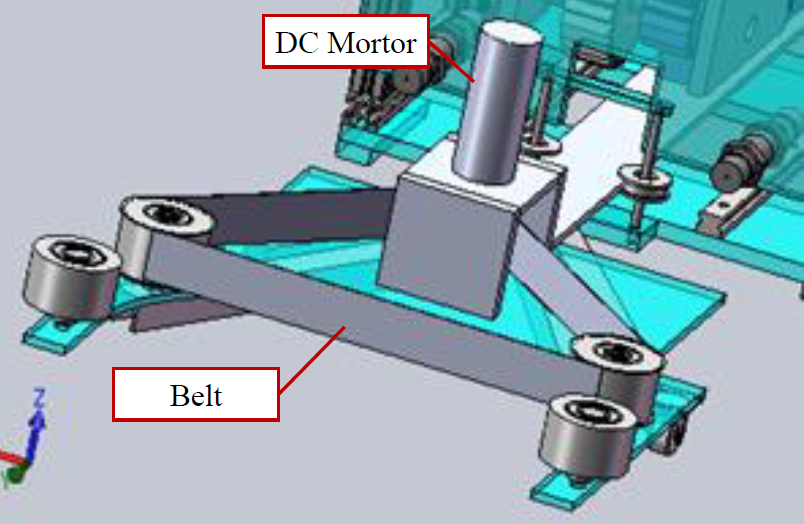
\includegraphics[width=\linewidth]{figures/1.png}
%         \caption{Flat belt type}
%         \label{fig:one}
%     \end{minipage}
%     \hfill
%     \begin{minipage}{0.4\linewidth}
%         \centering
%         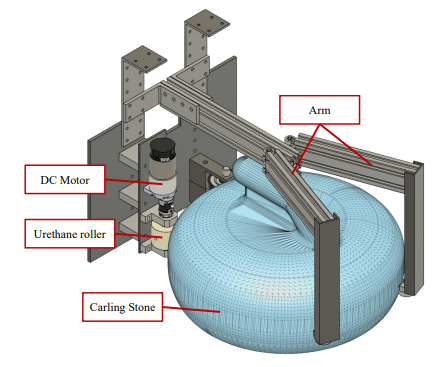
\includegraphics[width=\linewidth]{figures/2.png}
%         \caption{Urethane roller type}
%         \label{fig:two}
%     \end{minipage}
%     \hfill
%     \begin{minipage}{0.4\linewidth}
%         \centering
%         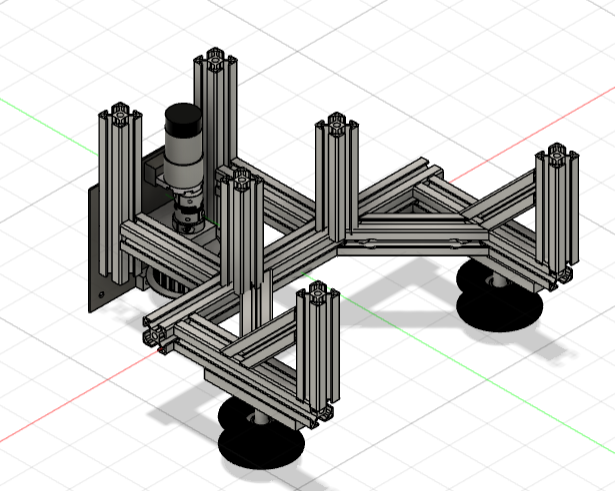
\includegraphics[width=\linewidth]{figures/3.png}
%         \caption{Timing belt type rotary}
%         \label{fig:three}
%     \end{minipage}
%     \vspace{0pt} % 上部の余白を0に設定
% \end{figure}
\subsection{新型回転付加機構の開発}
新たな回転付加機構について述べる.
先行研究で発覚した問題を新たな回転付加の設計を行うことで解決を図った.
現在設計を行っている回転付加機構のCAD図を図\ref{fig:new}に示す.
問題解決のため、カーリングストーンのハンドルを把持する機構を用いて、ハンドルを用いて回転を与えることで、問題であった確実な回転を付与することを目指す.
投球の際には,ボールスプラインを利用し、ハンドル把持部を上下させ、ストーンのハンドル部分との接触を外しストーンの投球を行う.
\begin{figure}[H]
    \centering
    \begin{minipage}{0.6\linewidth}
        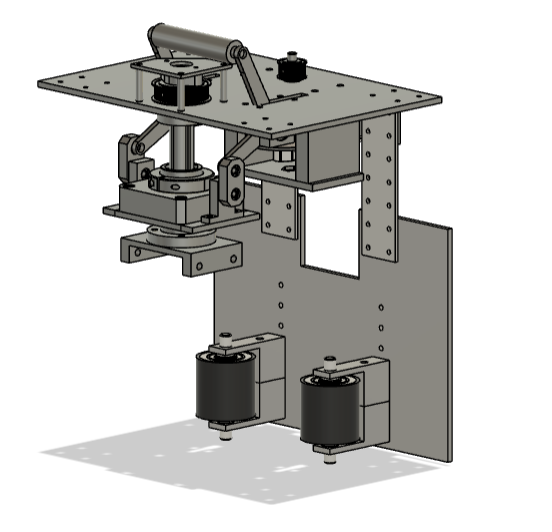
\includegraphics[width=\linewidth]{figures/4.png}
        \caption{New rotary addition mechanism}
        \label{fig:new}
    \end{minipage}
    \hfill
    \vspace{0pt} % 上部の余白を0に設定
\end{figure}



\section{まとめと今後の展望}
先行研究の回転付加機構の問題である確実な回転が付与が困難である問題を解決するため,
カーリングストーンのハンドル部分を把持し、ハンドル部分から回転を与える新型回転付加機構の設計を行った。
今後は,設計した回転付加機構をデリバリロボットに実装し,実験を行い回転付加機構の目標を達成することを目指す.



\printbibliography[title=参考文献]





\end{document}